\begin{Aufgabe}[10]
Hinweis: Alle Teilaufgaben können unabhängig voneinander bearbeitet werden.

\begin{enumerate}
	\item
	Ordnen Sie den Differenzialgleichungen die Richtungsfelder zu:

\begin{tabular}{p{0.25\textwidth}p{0.25\textwidth}p{0.25\textwidth}p{0.25\textwidth}}
	(A) $y' = -y$ &
	(B) $y' = -x$ &
	(C) $y' = y^2$ &
	(D) $y' = x^2$ \\
\end{tabular}

\begin{tabular}{llll}
	\ifLoesung
	( {\textcolor{red}C} ) &
	\else
	( \quad ) &
	\fi
	\hspace*{-10mm} \raisebox{-0.8\height}{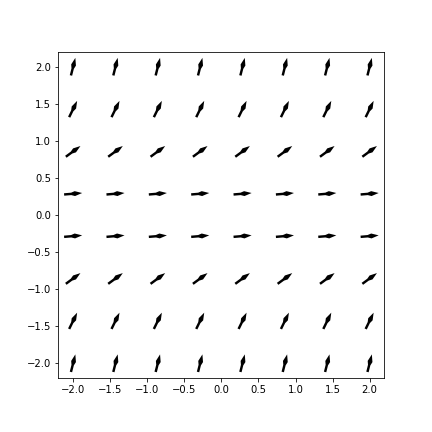
\includegraphics[width=0.4\textwidth]{../M2_IT/m2_it_ss_23_kurzaufgaben_richtungsfeld_3.png}} &
	\ifLoesung
	( {\textcolor{red}B} ) &
	\else
	( \quad ) &
	\fi
	\hspace*{-10mm} \raisebox{-0.8\height}{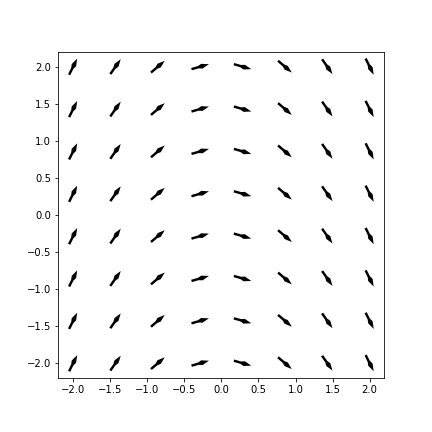
\includegraphics[width=0.4\textwidth]{../M2_IT/m2_it_ss_23_kurzaufgaben_richtungsfeld_2.png}}  \\
	\ifLoesung
	( {\textcolor{red}D} ) &
	\else
	( \quad ) &
	\fi
	\hspace*{-10mm} \raisebox{-0.8\height}{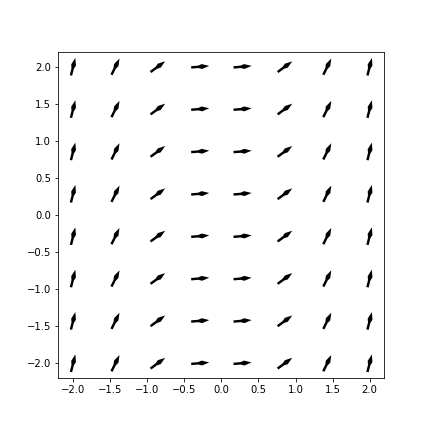
\includegraphics[width=0.4\textwidth]{../M2_IT/m2_it_ss_23_kurzaufgaben_richtungsfeld_4.png}} &
	\ifLoesung
	( {\textcolor{red}A} ) &
	\else
	( \quad ) &
	\fi
	\hspace*{-10mm} \raisebox{-0.8\height}{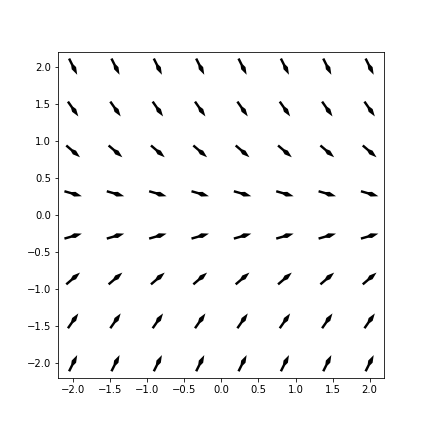
\includegraphics[width=0.4\textwidth]{../M2_IT/m2_it_ss_23_kurzaufgaben_richtungsfeld_1.png}}  \\
\end{tabular}

\ifLoesung
\mbox{}\hfill\Punkte{2 P}\\
\fi	

\pagebreak

	\item
		Welche Differenzialgleichung ist linear? Bitte kreuzen Sie den entsprechenden Eintrag an:

\ifLoesung 
\begin{tabular}{p{0.3\textwidth}p{0.2\textwidth}p{0.2\textwidth}}
	$y'' + 2 \, y' + y = \sin(x)$     & {\textcolor{red}X} linear &            $\square$ nicht linear\\
	$y'' + 2 \, y' + \sin(y) = 0$    & $\square$ linear  & {\textcolor{red}X} nicht linear\\
	$y'' + 2 \, y' + \sin(x) = 0$ &  {\textcolor{red}X} linear &            $\square$ nicht linear\\
	$y'' + 2 \, y' + \sin(x) \, y = 0$     & {\textcolor{red}X} linear &            $\square$ nicht linear\\
\end{tabular}
\hfill\Punkte{2 P}
\else
\begin{tabular}{p{0.3\textwidth}p{0.2\textwidth}p{0.2\textwidth}}
	$y'' + 2 \, y' + y = \sin(x)$     & $\square$ linear & $\square$ nicht linear\\
	$y'' + 2 \, y' + \sin(y) = 0$        & $\square$ linear & $\square$ nicht linear\\
	$y'' + 2 \, y' + \sin(x) = 0$     & $\square$ linear & $\square$ nicht linear\\
	$y'' + 2 \, y' + \sin(x) \, y = 0$ & $\square$ linear & $\square$ nicht linear\\
\end{tabular}
\fi

	\item
	Die Differenzialgleichung der Balkendurchbiegung $w(x)$ lautet:
	\[
		\frac{w''(x)}{({1 + (w'(x))^2})^{3/2}} = -\frac{M_y(x)}{E \, I_y} \, .
	\]
	Dabei bezeichnet $M_y(x)$ das Biegemoment an der Stelle $x$, $E$ das Elastizitätsmodul des Balkenmaterials und $I_y$ das axiale Flächenträgheitsmoment des Balkenquerschnitts.
	Stellen Sie die Differenzialgleichung mit Zustandsvariablen durch ein äquivalentes System von Differenzialgleichungen erster Ordnung dar.

\Loesung{}{
	Zwei Zustandsvariablen:
	\hfill\Punkte{2 P}
	\[
	z_1 = w(x), \, z_2 = w'(x) \, .
	\]
	System von Differenzialgleichungen erster Ordnung:
	\[
	\begin{array}{ccl}
		z'_1 & = & z_2 \, , \\
		z'_2 & = &  -\frac{M_y(x)}{E \, I_y} ({1 + z_2^2})^{3/2} \, .
	\end{array}
	\]
}
	
\pagebreak

	\item
		Folgende Frage wurde ChatGPT in der Version vom 12. Mai 2023 gestellt: 
		
		\begin{verbatim}
		Ein Teich enthält 1000 Liter Wasser. Täglich verdunsten 2% des Wassers im Teich und
		10 Liter Wasser werden nachgefüllt. Wieviel Wasser enthält der Teich nach 2 Tagen?
		\end{verbatim}
		
		Die Antwort lautete:
		
		\begin{verbatim}
		Zuerst berechnen wir die tägliche Verdunstungsmenge: 2% von 1000 Litern sind 20
		Liter. Da täglich 10 Liter Wasser nachgefüllt werden, verringert sich die Wasser-
		standsmenge um 10 Liter - 20 Liter = -10 Liter pro Tag. Nach 2 Tagen würde sich die
		Wassermenge im Teich um -10 Liter * 2 Tage = -20 Liter verringern. Da der Wasser-
		verlust die Nachfüllung übersteigt, enthält der Teich nach 2 Tagen kein Wasser mehr.
		\end{verbatim}
		
		Bestimmen Sie die korrekte Wassermenge im Teich nach $2$ Tagen mithilfe einer Differenzengleichung.
		
		\Loesung{5cm}{
			Differenzengleichung:
			\hfill\Punkte{2 P}
			\[
				T_{k+1} = 0.98 \, T_k + 10, \quad T_0 = 1000
			\]
			Nach einem Tag:
			\[
				T_1 = 0.98 \cdot 1000 + 10 = 990 
			\]
			Nach zwei Tagen:
			\[
				T_2 = 0.98 \cdot 990 + 10 =  980.2
			\]
			}
		
		\item
		Welchen Grenzwert $S$ hat die Reihe
		\[
			S = \sum_{k=2}^\infty \left(\frac{1}{3}\right)^k \, ?
		\]
		\Loesung{}{
			Geometrische Reihe mit $q = \frac{1}{3}$:
			\hfill\Punkte{2 P}
			\[
			\sum_{k=0}^\infty \left(\frac{1}{3}\right)^k  = \frac{1}{1 - q} = \frac{1}{1 - \frac{1}{3}} = \frac{3}{2} \, .
			\]
			Erste beiden Glieder:
			\[
				S = \sum_{k=2}^\infty \left(\frac{1}{3}\right)^k  = \sum_{k=0}^\infty \left(\frac{1}{3}\right)^k  - \left( 1 + \frac{1}{3} \right)  =   \frac{1}{6} 
			\]
		}
	\end{enumerate}

\end{Aufgabe}

\newpage

\endinput